\section{Experiments}
\label{sec:experiments}
In this section, we evaluate our method, MMFP, primarily compared to (i) Denoising Diffusion Probabilistic Models (DDPM)~\cite{ho2020denoising}, (ii) Flow Matching (FM)~\cite{lipman2022flow}, (iii) Task-Conditional Variational Autoencoder (TCVAE) with a Gaussian prior~\cite{noseworthy2020task}, and (iv) Motion Manifold Primitives with a Gaussian mixture prior (MMP)~\cite{lee2023equivariant}.  
DDPM and FM are directly trained in the trajectory space \(\mathcal{X}\). When \(\mathcal{X} = \mathrm{SE}(3)^T\), a Riemannian manifold, we train a DDPM in local coordinates (using exponential coordinates for the $\mathrm{SO}(3)$ component) and use Riemannian Flow Matching (RFM)~\cite{chen2023riemannian}.  
MMFP trained without the robustness regularization term (the second term in (\ref{eq:lfl})) will be denoted as MMFP w/o reg.

For MMFP, we choose the latent space dimension $m=3$ for ${\cal Z} = \mathbb{R}^{m}$ and text embedding dimension $p=3$ for ${\cal T}=\mathbb{R}^{p}$. For TCVAE and MMP, with thorough tuning, we set the latent space dimension to be $3$ or $4$ and text embedding dimension to be $64$.
We compare models for 6-DoF SE(3) pouring trajectory generation and 7-DoF robot arm waving motion generation tasks. 
Throughout, we use fully-connected neural networks with ELU activation functions.

\textbf{Evaluation metrics:} {The primary objective is to generate correct motions corresponding to the given text inputs. To evaluate whether the model generates accurate motions that perform the task described in the given text, we train a trajectory classifier and use it to report the motion accuracy; the higher, the better. 
Additionally, the model should be able to generate not just a single trajectory but diverse trajectories, imitated from the given demonstration dataset, depending on the text input. For example, see Fig.~\ref{fig:diverse_pouring_motion_corl}. 
We use the Maximum Mean Discrepancy (MMD)~\cite{gretton2012kernel} -- which measures the distance between two probability distributions, computed from their samples -- to measure the similarity between the set of generated trajectories given a text input and the set of demonstration trajectories annotated with that text; the lower, the better. 

Texts are annotated to each trajectory at multiple different levels (e.g., see Fig.~\ref{fig:pouring_dataset_and_results_corl} {\it Left} and Fig.~\ref{fig:dataset_waving} {\it Left}), with higher levels specifying more detailed requirements. Multiple trajectories can correspond to the same text (e.g., all trajectories being assigned the same level 1 text), resulting in many-to-many text-motion correspondences.
The MMD metrics are measured separately for each level text input, then averaged across text descriptions at the same level. 
Evaluation metrics are computed using both seen and unseen texts in training. First, accuracy and MMD metrics are measured using the seen texts. Then, to evaluate the robustness to text variations, we also report robust MMD metrics, which are computed with unseen text inputs generated by ChatGPT.

We begin this section by comparing latent diffusion and flow matching models on text-based 2D motion generation tasks. We then present experiments involving higher-dimensional configuration spaces, including text-based SE(3) pouring motion generation and 7-DoF waving motion generation tasks.

\subsection{Latent diffusion vs latent flow matching}
\label{sec:toy_exp}
In this section, using the simple 2D trajectory generation task shown in Fig.~\ref{fig:toy_data}, we compare our motion manifold flow primitives trained with latent flow matching models to those trained with latent diffusion models~\cite{song2020score}, denoted as MMP + Diffusion, while using the same motion manifold (an autoencoder). 

The dataset consists of 20 demonstration trajectories, all starting from the same point and ending at a common goal (the origin). Each trajectory has a length of $T=201$. For each trajectory, two text annotations are provided (see Fig.~\ref{fig:toy_data}). 

Diffusion models involve several design choices~\cite{song2020denoising}: the diffusion paths and noise schedules. In this experiment, latent diffusion models are trained using various Gaussian probability paths, including the variance-exploding path, denoted as Diffusion-VE, and two variance-preserving paths with different noise schedules, denoted as Diffusion-VP-1 and Diffusion-VP-2.

As shown in Table~\ref{tab:main_toy_extended} and Fig.~\ref{fig:appendix_dif_vs_ot}, MMFP achieves strong performance across both levels of text inputs simultaneously. In contrast, MMP combined with diffusion models yields less satisfactory results, performing well on either the level 1 or level 2 task but failing to achieve strong performance on both simultaneously.
These results can be attributed to the smoother optimal transport paths~\cite{lipman2022flow} used in flow matching compared to diffusion paths. These smoother paths simplify the underlying ground-truth vector field that the neural network vector field \(v_s(z,c)\) needs to fit, making the fitting process easier, improving accuracy, and reducing the number of function evaluations required during sampling.

\begin{figure}[!t]
    \centering
    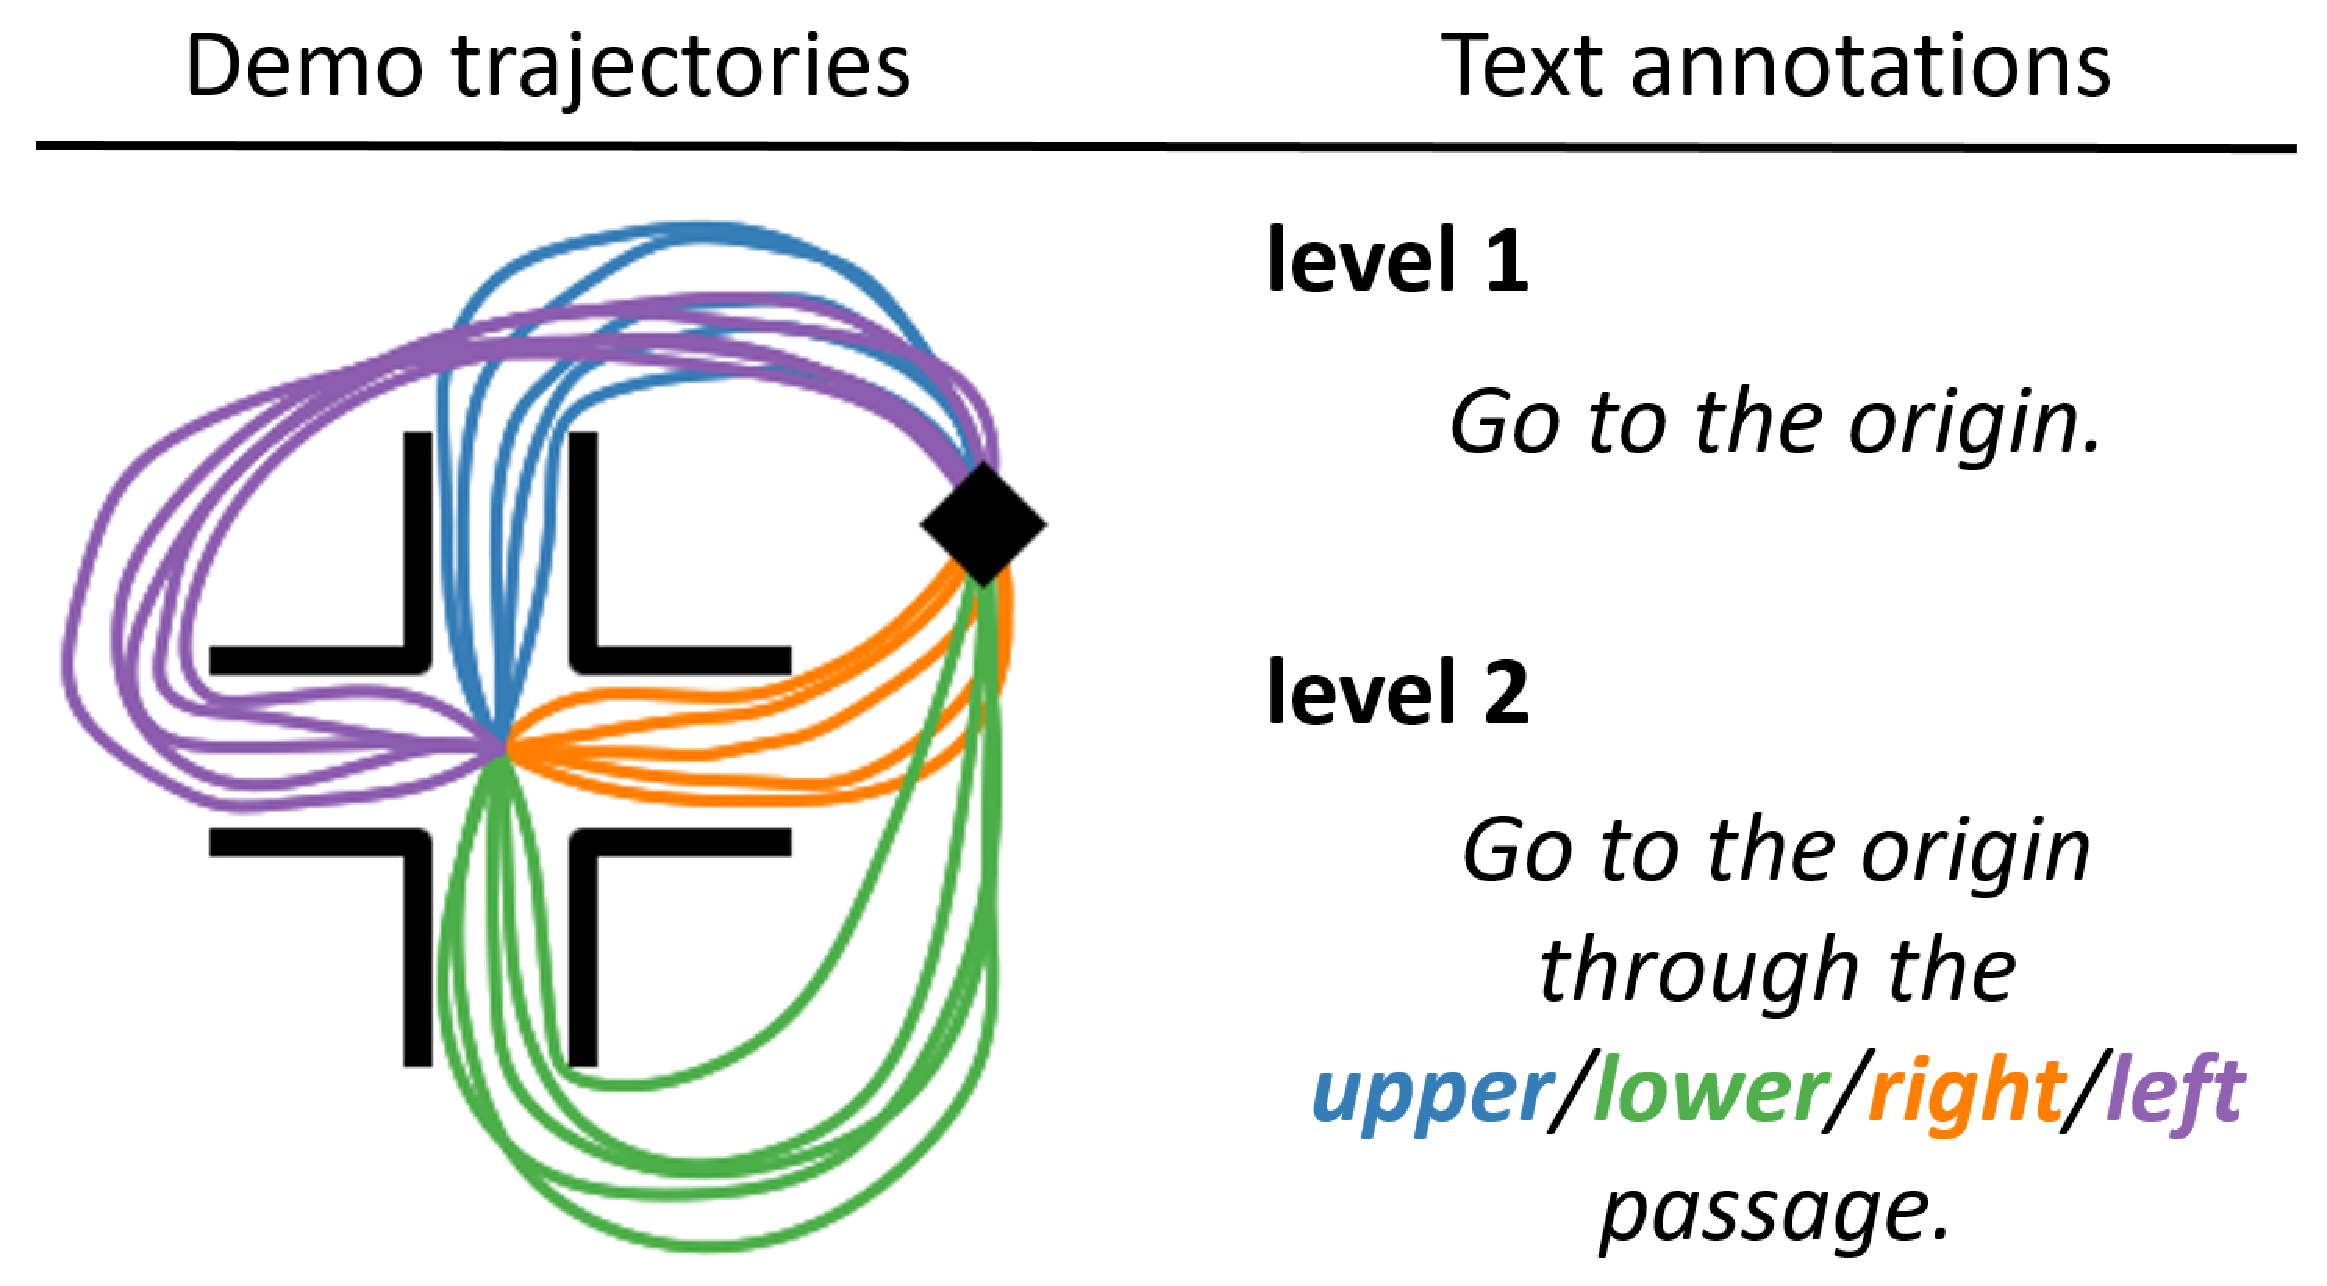
\includegraphics[width=0.3\textwidth]{tabs/figures/ral_toy_data2.pdf}
    \caption{Demonstration trajectories with multiple text annotations. Each trajectory is assigned with two text labels, the level 1 and level 2 texts.}
    \label{fig:toy_data}
\end{figure}

\begin{table}[!t]
\centering
\scriptsize
\caption{The MMD metric and accuracy ($\%$) for 2D motion generation.}
\label{tab:main_toy_extended}
\begin{tabular}{ccccc} 
\toprule
& \multicolumn{2}{c}{MMD ($\downarrow$)}  & \multicolumn{2}{c}{Accuracy ($\uparrow$)}  \\ \cmidrule(lr){2-3} \cmidrule(lr){4-5} 
& level 1 & level 2 & \begin{tabular}[c]{@{}c@{}} path \end{tabular} & task \\ 
                                                           \midrule
\begin{tabular}[c]{@{}c@{}}MMP + Diffusion-VE \end{tabular}  & 0.075 & {\bf 0.007} & 100 & 94.6 \\
\begin{tabular}[c]{@{}c@{}}MMP + Diffusion-VP-1 \end{tabular} & 0.073 & {\bf 0.003} & 100 & 95.0   \\
\begin{tabular}[c]{@{}c@{}}MMP + Diffusion-VP-2 \end{tabular} & {\bf 0.030} & 0.055 & 94.3 & 81.0   \\
\begin{tabular}[c]{@{}c@{}}MMFP \end{tabular}  & {\bf 0.025} & {\bf 0.004} & {\bf 100} & {\bf 99.8}   \\
\bottomrule
\end{tabular}
\end{table}

\begin{figure}[!t]
    \centering
    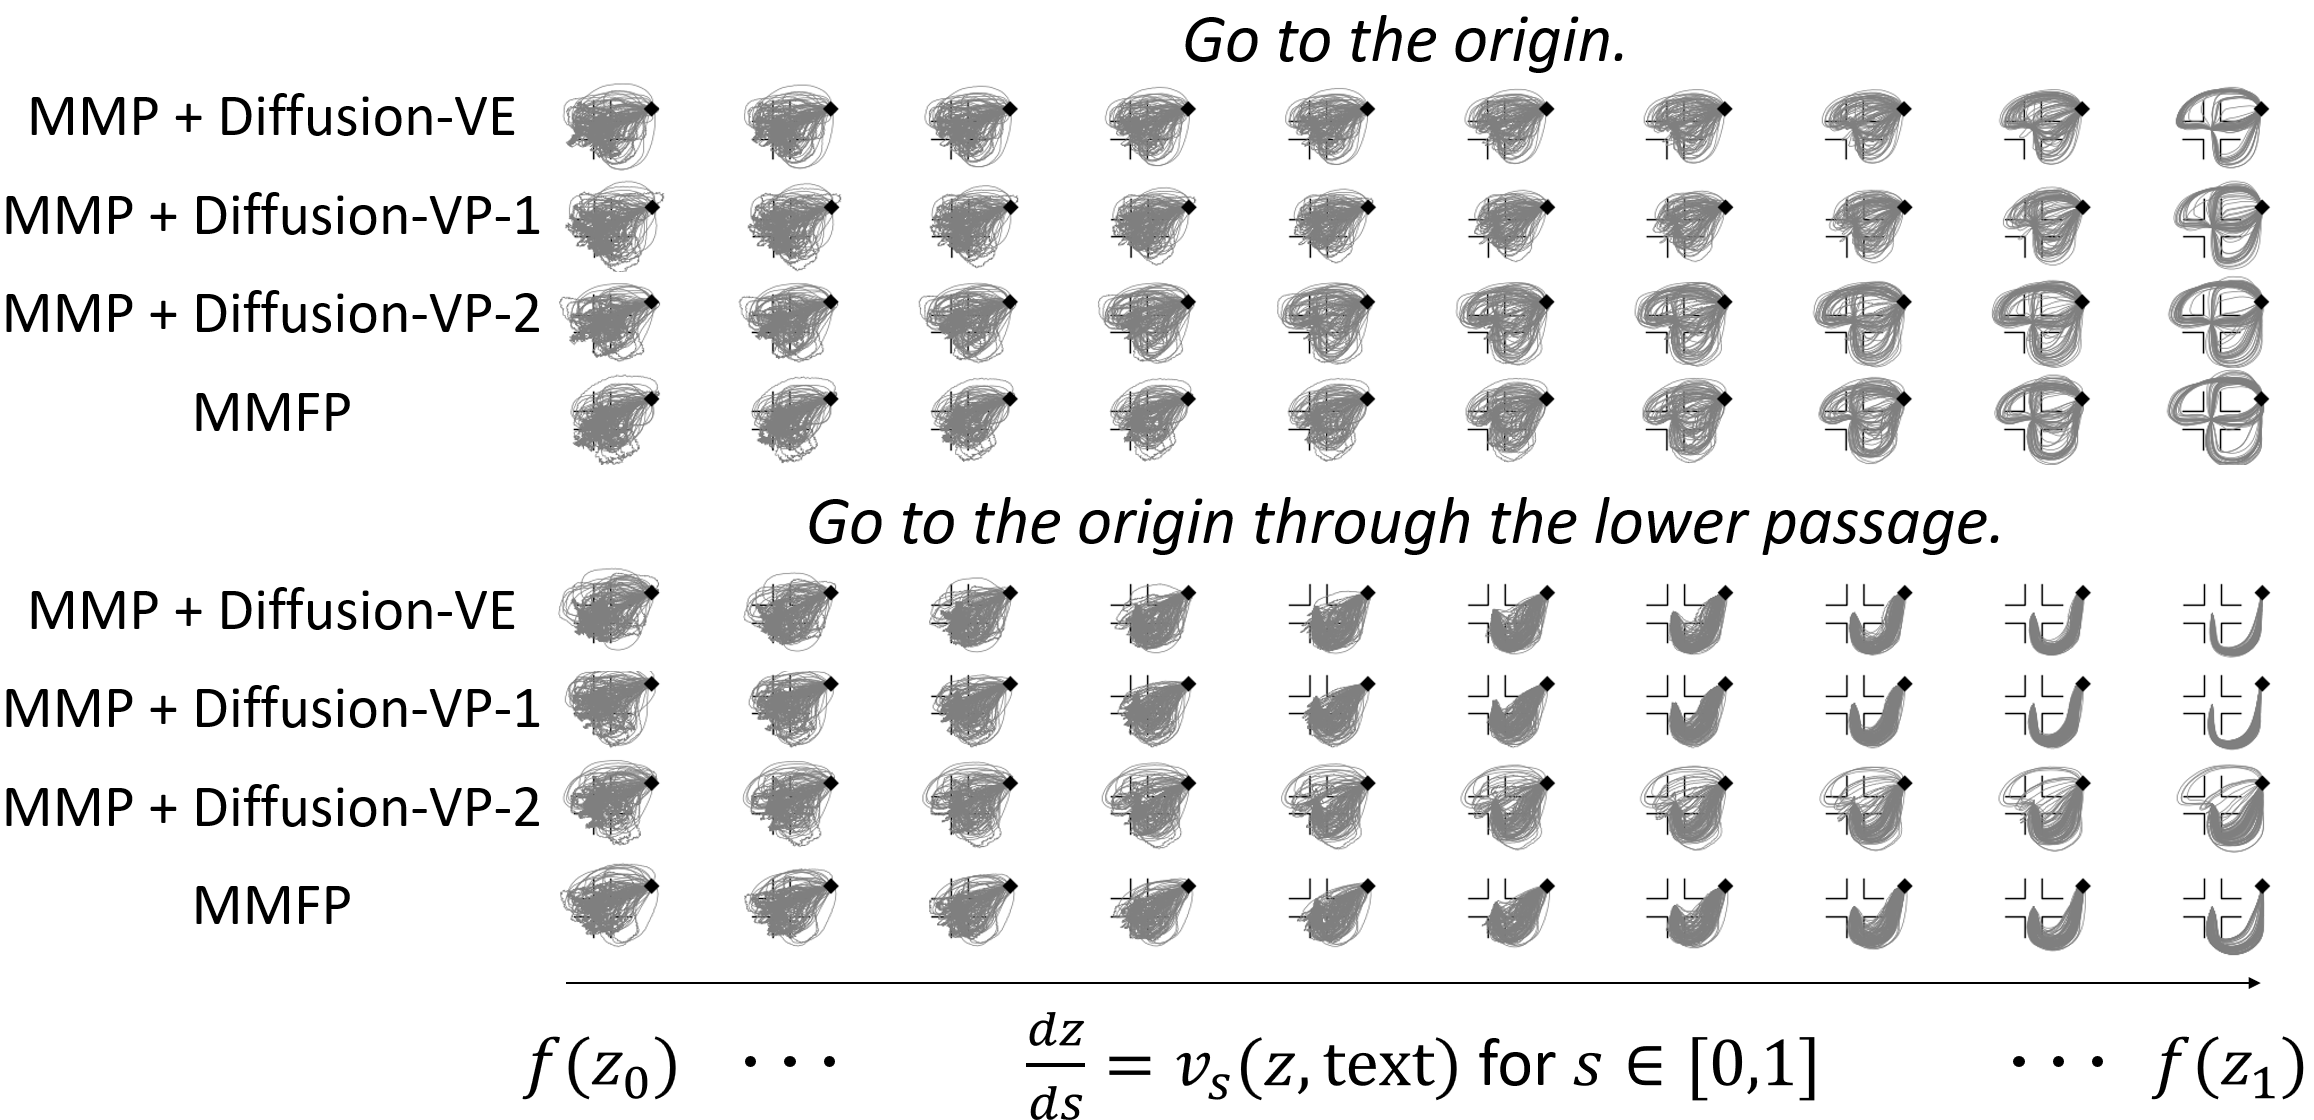
\includegraphics[width=1\linewidth]{tabs/figures/ral_2d_toy_results.png}
    \caption{The evolution of generated trajectories (from left to right) follows each of the latent models, either diffusion or flow, with the trajectories on the far right representing the final output samples.}
    \label{fig:appendix_dif_vs_ot}
\end{figure}



\subsection{SE(3) pouring motion generation}

\begin{table*}[!t]
\scriptsize
\centering
\caption{The MMD and robust MMD metrics and the accuracy ($\%$) for pouring motion generation.}
\label{tab:main}
\begin{tabular}{lccccccccc} 
\toprule
& \multicolumn{3}{c}{MMD ($\downarrow$)}    & \multicolumn{3}{c}{robust MMD ($\downarrow$)} & \multicolumn{3}{c}{Accuracy ($\uparrow$)}  \\ 
\cmidrule(lr){2-4} \cmidrule(lr){5-7} \cmidrule(lr){8-10}
& level 1 & level 2 & level 3 & level 1   & level 2  & level 3  & \begin{tabular}[c]{@{}c@{}}pouring \\ style\end{tabular} & \begin{tabular}[c]{@{}c@{}}pouring \\ direction\end{tabular} & both \\ 
\midrule
DDPM~\cite{ho2020denoising} & 0.398 & 0.484 & 1.306 & 0.400 & 0.486 & 1.304 & 50.5 & 20.0 & 10.2\\
RFM~\cite{chen2023riemannian}   & 0.411 & 0.431 &	0.778 &	0.413 &	0.425 &	1.127 & 87.0 & 36.4 & 30.8 \\
TCVAE~\cite{noseworthy2020task} & 0.117 & 0.211 & 0.824 & 0.131 & 0.191 & 1.041 & 52.0 & 25.4 & 15.3 \\
MMP~\cite{lee2023equivariant}  & {\bf 0.045} & {\bf 0.115} & 0.950 & {\bf 0.055} & {\bf 0.112} & 0.970 & 47.5 & 19.6 & 9.3 \\
\begin{tabular}[c]{@{}c@{}} MMFP w/o reg (ours) \end{tabular} 
      & {\bf 0.055}  & {\bf 0.114} & {\bf 0.009} & {\bf 0.056} & {\bf 0.097} & 0.096 & {\bf 98.5} & {\bf 93.2} & {\bf 99.9} \\
\begin{tabular}[c]{@{}c@{}} MMFP (ours) \end{tabular} 
      & {\bf 0.042}  & {\bf 0.093} & {\bf 0.007} & {\bf 0.052} & {\bf 0.094} & {\bf 0.016} & {\bf 99.0} & {\bf 92.6} & {\bf 99.9} \\
\bottomrule
\end{tabular} 
\end{table*}

\begin{figure*}[!t]
    \centering
    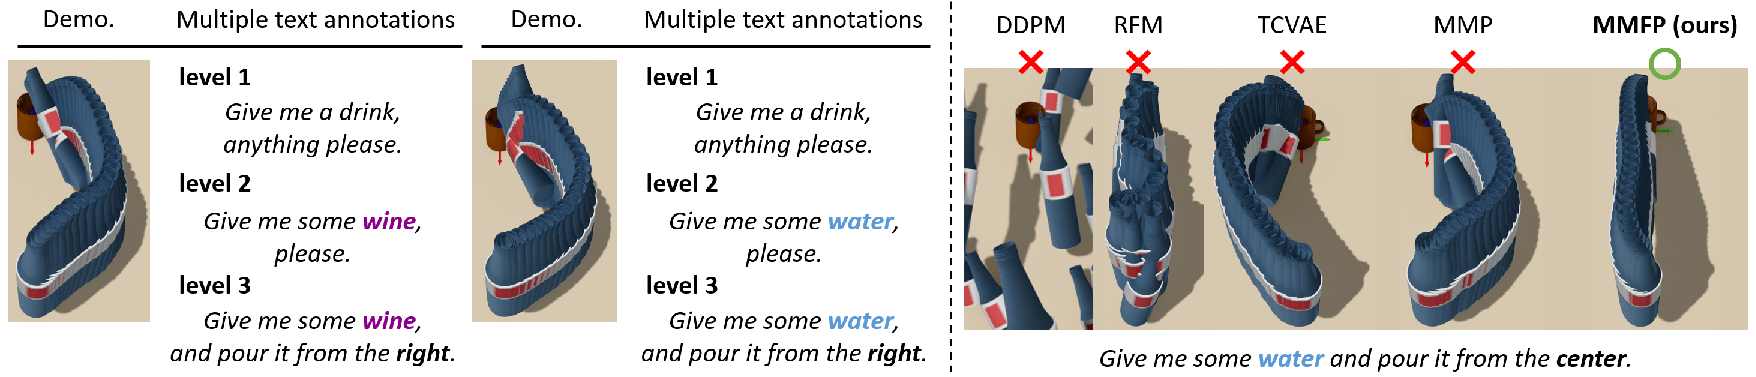
\includegraphics[width=1\linewidth]{tabs/figures/ral_pouring_dataset_and_results.pdf}
    \caption{{\it Left}: Example demonstration trajectories, each of which is annotated with three different level texts. {\it Right}: Generated pouring trajectories by RFM, TCVAE, MMP and MMFP.}
    \label{fig:pouring_dataset_and_results_corl}
\end{figure*}

\begin{figure*}[!t]
    \centering
    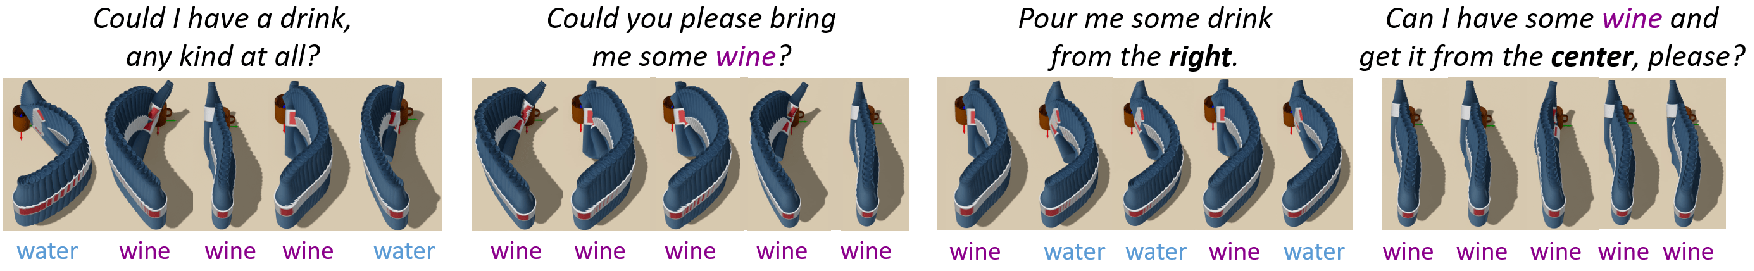
\includegraphics[width=1\linewidth]{tabs/figures/ral_diverse_pouring_motion.pdf}
    \caption{A variety of accurate trajectories generated by MMFP given unbiased text inputs.}
    \label{fig:diverse_pouring_motion_corl}
\end{figure*}

\begin{figure}[!t]
    \centering
    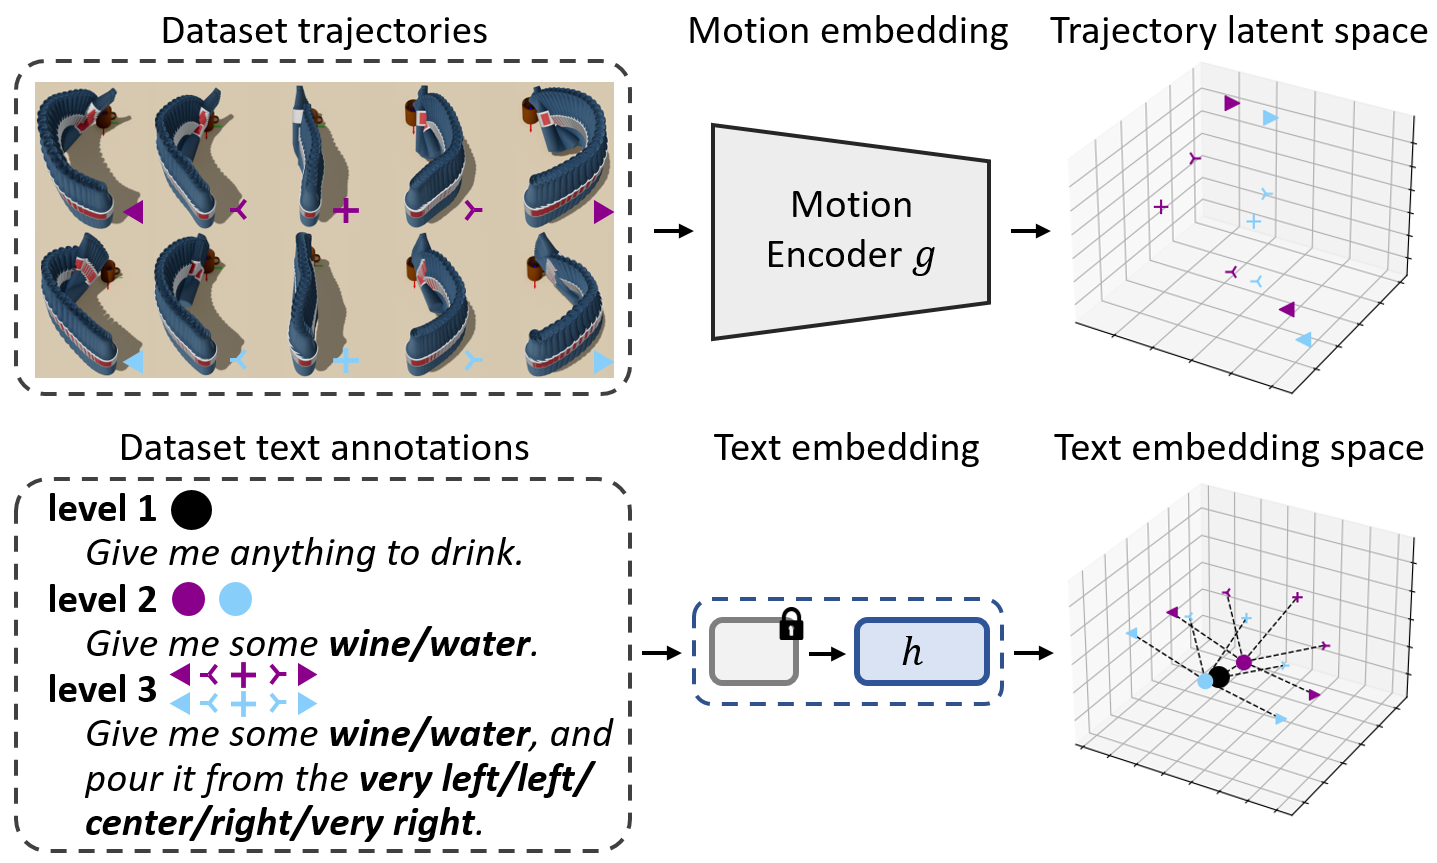
\includegraphics[width=1\linewidth]{tabs/figures/ral_visual_analysis.PNG}
    \caption{{\it Upper}: SE(3) pouring trajectory data encoded in the three-dimensional latent space by our motion encoder. {\it Lower}: Texts used in training encoded in the three-dimensional text embedding space by our text embedding model.}
    \label{fig:results1-label}
\end{figure}

\begin{figure}[!t]
    \centering
    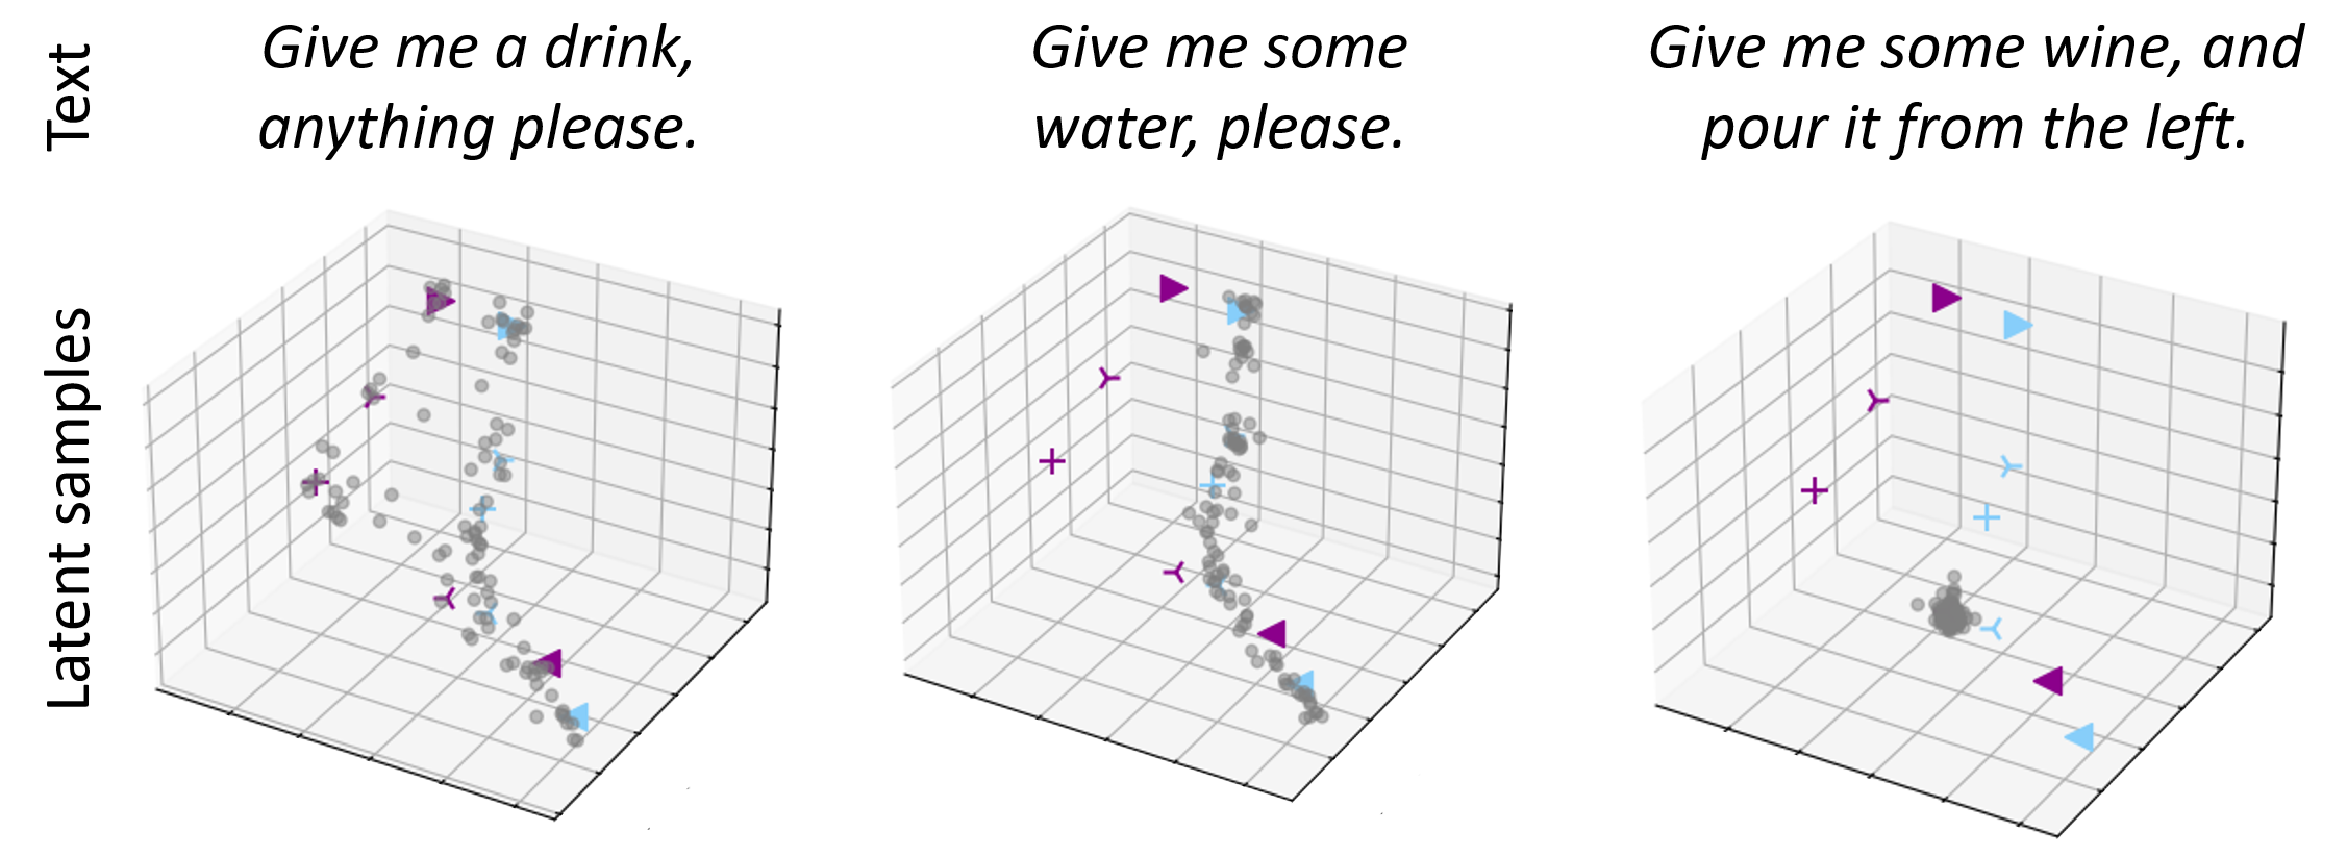
\includegraphics[width=1\linewidth]{tabs/figures/ral_results2.pdf}
    \caption{Sampled latent points by our trained latent flow model in MMFP. {\it Left}: Sampled latent points given the level 1 text. {\it Middle}: Sampled latent point given a level 2 text. {\it Right}: Sampled latent points given a level 3 text.}
    \label{fig:results2-label}
\end{figure}

\begin{figure}[!t]
    \centering
    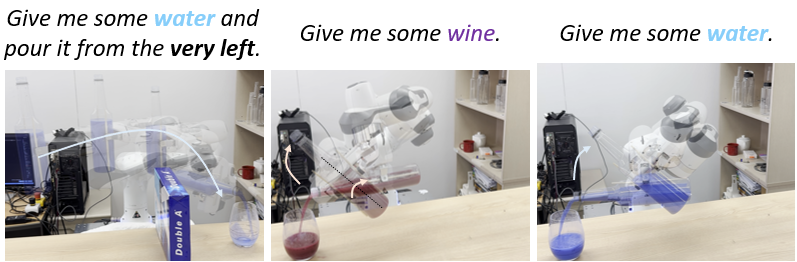
\includegraphics[width=1\linewidth]{tabs/figures/ral_pouring_real.png}
    \caption{Real robot pouring motion generation results.}
    \label{fig:real_exp}
\end{figure}

In this section, we train text-based pouring motion generation models, where the dataset is obtained from the human demonstration videos. 
The demonstrator is instructed to pour water or wine in five different pouring directions (i.e., from the very left, left, center, right, and very right side). When pouring wine, the demonstrator is instructed to turn the wrist clockwise at the end.
From ten videos, we extract SE(3) trajectories of the bottles, and the trajectory lengths are pre-processed so that $T=480$. 
For each trajectory, we give three text annotations, as shown in Fig.~\ref{fig:pouring_dataset_and_results_corl} ({\it Left}). 
Notably, multiple trajectories can be associated with a single text label, leading to many-to-many correspondences between text and motion. For example, all 10 trajectories are labeled with the level 1 text, ``Give me a drink, anything please''.

Table~\ref{tab:main} shows MMD, robust MMD, and Accuracy; our MMFP only shows good scores in all metrics. We note that the regularization in MMFP significantly improves the level 3 robust MMD metric. 
The DDPM and RFM overall produce very poor MMD results. As shown in Fig.~\ref{fig:pouring_dataset_and_results_corl} ({\it Right}), the trajectory generated by DDPM does not even converge near the cup and that of RFM is very jerky. 
TCVAE and MMP, both adopting the motion manifold hypothesis, produce motions of reasonable quality. 
Nevertheless, they exhibit a limitation in understanding level 3 text descriptions, particularly regarding pouring directions. 
Examples illustrating this limitation can be observed in Fig.~\ref{fig:pouring_dataset_and_results_corl} ({\it Right}), where they fail in pouring from accurate directions. Lastly, Fig.~\ref{fig:diverse_pouring_motion_corl} shows a variety of accurately generated motions by MMFP given unbiased user text inputs not seen during training.

Furthermore, we present a visual analysis of our MMFP, wherein the three-dimensional nature of both the latent space \(\mathcal{Z}\) and the text embedding space \(\mathcal{T}\) facilitates straightforward visualization. 
Fig.~\ref{fig:results1-label} ({\it Upper}) shows the latent values of the trajectory data, i.e., \(z^i = g(x^i) \in \mathbb{R}^{3}\), where \(g\) is a trained encoder.  
Fig.~\ref{fig:results1-label} ({\it Lower}) displays the embedding vectors of the text inputs, i.e., \(\tau^i = h(c^i) \in \mathbb{R}^{3}\), where \(h\) is a trained text embedding module.
Semantically similar trajectories and texts are positioned closely together, exhibiting smooth transitions as their meanings shift, indicating successful model training.

Fig.~\ref{fig:results2-label} highlights the multi-modality of the text-conditioned latent distribution and, more importantly, the complex text-motion dependencies, as evidenced by the substantial shifts in the distribution with varying text inputs. In the figure, moving from left to right corresponds to scenarios where level 1 to level 3 texts are given as inputs. When a level 1 text is provided, the distribution must fit two modalities, and the volume of the distribution is the largest. In contrast, when level 2 or level 3 texts are provided, there is only one modality. Note that the support of the distribution varies significantly from level 1 to level 3, becoming much smaller at level 3.
This implies that a latent text-conditioned distribution should capture such dramatic changes, fitting a complex, non-smooth function. Existing manifold-based models relying on conditional autoencoders struggle to capture such a complex function, whereas our MMFP effectively models it.

Lastly, we conduct real robot experiments (see Fig.~\ref{fig:real_exp}). Given the generated SE(3) trajectories of the bottle, we compute joint space trajectories by solving the inverse kinematics. 
The generated SE(3) trajectory is smooth and densely discretized enough that, despite the relatively high speed of the bottle, the robot can accurately track the desired end-effector pose using computed torque control with a PD control law.

\subsection{7-DoF waving motion generation}
\begin{table*}[!t]
\centering
\scriptsize
\caption{The MMD and robust MMD metrics and the accuracy ($\%$) for waving motion generation.}
\label{tab:main_waving}
\begin{tabular}{lccccccccc} 
\toprule
& \multicolumn{3}{c}{MMD ($\downarrow$)}    & \multicolumn{3}{c}{robust MMD ($\downarrow$)} & \multicolumn{3}{c}{Accuracy ($\uparrow$)}  \\ 
\cmidrule(lr){2-4} \cmidrule(lr){5-7} \cmidrule(lr){8-10}
& level 1 & level 2 & level 3 & level 1   & level 2  & level 3  & \begin{tabular}[c]{@{}c@{}}waving \\ direction\end{tabular} & \begin{tabular}[c]{@{}c@{}}waving \\ style\end{tabular} & both \\ 
\midrule
DDPM~\cite{ho2020denoising} & 0.425 & 0.542 & 0.831 & 0.427 & 0.542 & 0.831 & 18.4 & 29.3 & 4.1 \\
FM~\cite{lipman2022flow}  & 0.211 & 0.368 & 0.646 & 0.215 & 0.384 & 0.671 & {\bf 99.6} & 88.7 & 91.1 \\
TCVAE~\cite{noseworthy2020task} & 0.269 & 0.581 & 0.833 & 0.294 & 0.606 & 0.865 & 25.6 & 57.3 & 10.7 \\
MMP~\cite{lee2023equivariant} & {\bf 0.013} & 0.369 & 0.772 & {\bf 0.016} & 0.355 & 0.750 & 19.2 & 30.7 & 6.5\\
\begin{tabular}[c]{@{}c@{}} MMFP w/o reg (ours) \end{tabular} 
      & {\bf 0.020} & {\bf 0.037} & {\bf 0.006} & {\bf 0.024} & {\bf 0.046} & 0.021 & {\bf 99.8} & {\bf 98.7} & {\bf 99.7} \\
\begin{tabular}[c]{@{}c@{}} MMFP (ours) \end{tabular} 
      & {\bf 0.016} & {\bf 0.040} & {\bf 0.004} & {\bf 0.022} & {\bf 0.040} & {\bf 0.005} & {\bf 100} & {\bf 97.7} & {\bf 100} \\
\bottomrule
\end{tabular}
\end{table*}

\begin{figure*}[!t]
    \centering
    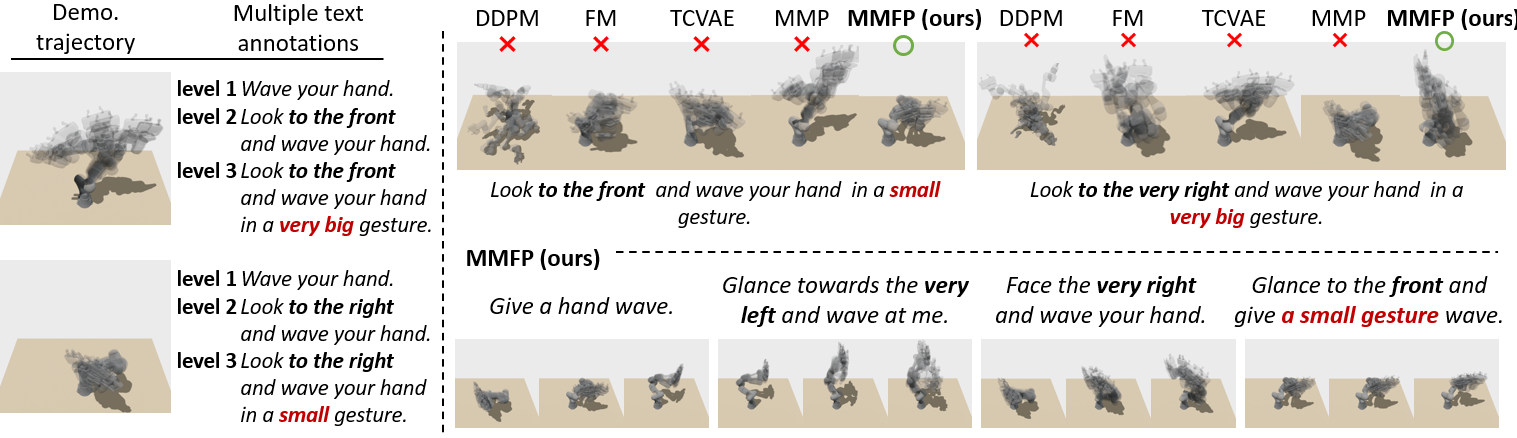
\includegraphics[width=1\linewidth]{tabs/figures/ral_waving_results.png}
    \caption{{\it Left}: Example 7-DoF demonstration trajectories, each of which is assigned with three different text labels. {\it Right-Upper}: Generated waving trajectories by DDPM, FM, TCVAE, MMP and MMFP. {\it Right-Lower}: A variety of accurate trajectories generated by MMFP given unbiased text inputs.}
    \label{fig:dataset_waving}
\end{figure*}

\begin{figure}[!t]
    \centering
    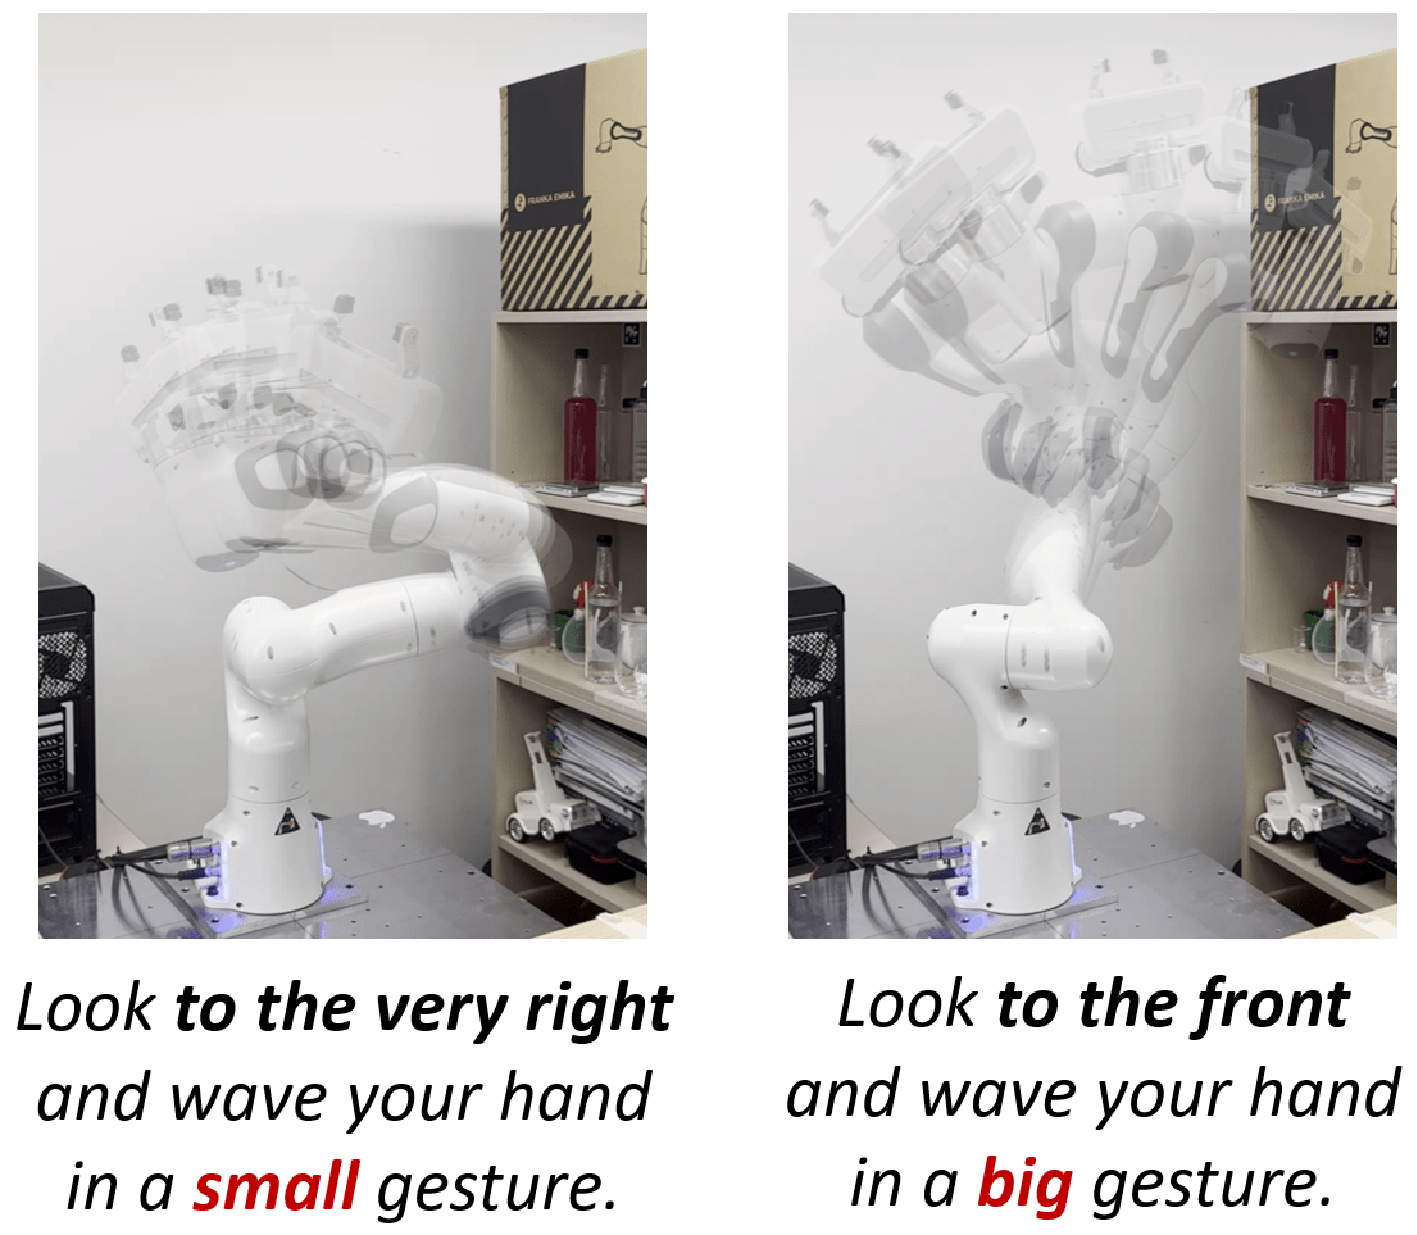
\includegraphics[width=0.6\linewidth]{tabs/figures/ral_real_waving_exp.pdf}
    \caption{Real robot waving motion generation by MMFP.}
    \label{fig:real_waving_exp_corl}
\end{figure}

In this section, we train text-based 7-DoF waving motion generation models, where the dataset is obtained from human demonstrations. The demonstrator is instructed to hold and move the robot arm so that the robot arm mimics waving motions in five different viewing directions (i.e., very left, left, front, right, and very right) and in three different styles (i.e., very big, big, small). We extract 7-DoF joint space trajectories, and the trajectory lengths are pre-processed to ensure $T=720$. 
Thus, ${\cal Q} = \mathbb{R}^{7}$, and the trajectory space is denoted as ${\cal X} = \mathbb{R}^{7 \times T}$. 
We encode two motions for each setting, resulting in a total of $N=30$ trajectories. For each trajectory, we provide three text annotations, as shown in Fig.~\ref{fig:dataset_waving} ({\it Left}). 

Table~\ref{tab:main_waving} presents the MMD, robust MMD, and Accuracy metrics, where MMFP once again achieves strong performance across all measures. These results align consistently with the findings from the previous pouring experiment. See Fig.~\ref{fig:dataset_waving} for qualitative results. Additionally, examples of real robot waving motion generated using our MMFP are illustrated in Fig.~\ref{fig:real_waving_exp_corl}.
